\documentclass[a4paper,11pt]{article}
\usepackage{amsmath,amssymb,color,comment}
\usepackage[compat=1.1.0]{tikz-feynhand}
\usepackage[T1]{fontenc}

\begin{document}

  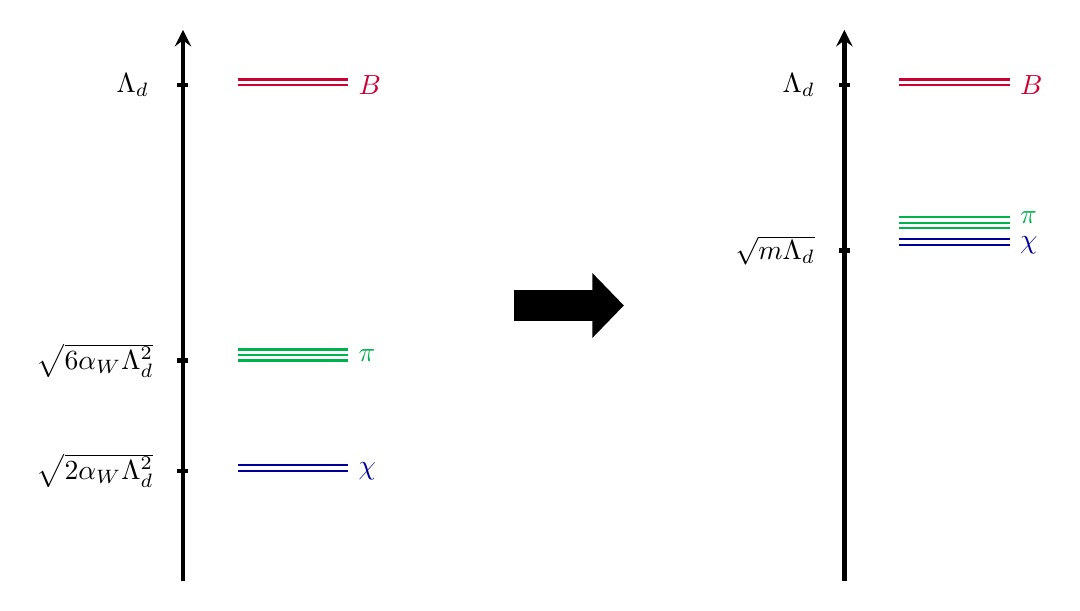
\begin{tikzpicture}[scale=0.7]
    \draw[->,>=stealth, ultra thick](-7,-5)--(-7,5);
    \draw[ultra thick] (-7.1,-3)--(-6.9,-3) node[left=0.3cm] {$\sqrt{2\alpha_W\Lambda_d^2}$};
    \draw[ultra thick] (-7.1,-1)--(-6.9,-1) node[left=0.3cm]{$\sqrt{6\alpha_W\Lambda_d^2}$};
    \draw[ultra thick] (-7.1,4)--(-6.9,4) node[left=0.3cm]{$\Lambda_d\,$};
    \draw[thick, red!80!blue] (-6,4)--(-4,4) node[right]{$B$};
    \draw[thick, red!80!blue] (-6,4.1)--(-4,4.1);
    \draw[thick, blue!30!green] (-6,-1)--(-4,-1) ;
    \draw[thick, blue!30!green] (-6,-0.9)--(-4,-0.9)node[right]{$\pi$};
    \draw[thick, blue!30!green] (-6,-0.8)--(-4,-0.8);
    \draw[thick, blue!60!black] (-6, -3)--(-4,-3) node[right]{$\chi$};
    \draw[thick, blue!60!black] (-6,-2.9)--(-4, -2.9);
    \draw[->,>={Triangle[width=8mm, length=4mm]}, line width=4mm] (-1,0)--(1,0);
    \draw[->,>=stealth, ultra thick](5,-5)--(5,5);
    \draw[ultra thick] (4.9,4)--(5.1,4) node[left=0.3cm]{$\Lambda_d$};
    \draw[ultra thick] (4.9,1)--(5.1,1) node[left=0.3cm]{$\sqrt{m\Lambda_d}$};
    \draw[thick, red!80!blue] (6,4)--(8,4) node[right]{$B$};
    \draw[thick, red!80!blue] (6,4.1)--(8,4.1);
    \draw[thick,blue!60!black] (6,1.1)--(8,1.1)node[right]{$\chi$};
    \draw[thick,blue!60!black] (6,1.2)--(8,1.2);
    \draw[thick, blue!30!green] (6,1.4)--(8,1.4);
    \draw[thick, blue!30!green] (6,1.5)--(8,1.5);
    \draw[thick, blue!30!green] (6,1.6)--(8,1.6)node[right]{$\pi$};
\end{tikzpicture}

\end{document}